\documentclass{article}
\usepackage{iclr2027_conference,times}

% Optional math commands from https://github.com/goodfeli/dlbook_notation.
\input{math_commands.tex}

\usepackage{url}
\usepackage{graphicx}
\usepackage{float}
\usepackage{capt-of}
\usepackage{wrapfig}
\usepackage{placeins}
\usepackage{multirow}
\usepackage{colortbl}
\usepackage{booktabs}
\usepackage{hyperref}

\setcounter{dbltopnumber}{3}
\renewcommand{\dbltopfraction}{0.95}
\setlength{\dblfloatsep}{4pt}

% Cell colors for the first-, second-, and third-ranked results in tables.
\definecolor{rankfirst}{RGB}{220,239,210}
\definecolor{ranksecond}{RGB}{255,246,196}
\definecolor{rankthird}{RGB}{207,230,240}
\newcommand{\first}[1]{\cellcolor{rankfirst}#1}
\newcommand{\second}[1]{\cellcolor{ranksecond}#1}
\newcommand{\third}[1]{\cellcolor{rankthird}#1}

\title{SplatAnything: \\ Gaussian Spacing Normalization for Feed-forward 3DGS across Arbitrary Scenes}

% Public preprint author list. Affiliations:
% 1: Zhejiang University; 2: Tencent Hunyuan; 3: Causa Robotics.
\author{%
\textbf{Hao Yu}$^{1,2}$ \quad
\textbf{Zhenwei Wang}$^{2}$ \quad
\textbf{Yongzhen Hu}$^{1}$ \quad
\textbf{Yuning Gong}$^{2}$ \quad
\textbf{Junta Wu}$^{2}$ \\
\textbf{Xiaowei Zhou}$^{1}$ \quad
\textbf{Hujun Bao}$^{1}$ \quad
\textbf{Tengfei Wang}$^{2,\dagger}$ \quad
\textbf{Chunchao Guo}$^{2,\dagger}$ \quad
\textbf{Sida Peng}$^{1,3}$ \\
$^{1}$Zhejiang University \quad
$^{2}$Tencent Hunyuan \quad
$^{3}$Causa Robotics \\
$^{\dagger}$Corresponding author%
}

% Show the public author list and suppress the ICLR review ruler. The document
% uses the plain page style below, so no conference-publication header is shown.
\iclrfinalcopy

\hypersetup{
  hidelinks,
  pdftitle={SplatAnything: Gaussian Spacing Normalization for Feed-forward 3DGS across Arbitrary Scenes},
  pdfauthor={Hao Yu, Zhenwei Wang, Yongzhen Hu, Yuning Gong, Junta Wu, Xiaowei Zhou, Hujun Bao, Tengfei Wang, Chunchao Guo, Sida Peng}
}

\begin{document}
\pagestyle{plain}
\raggedbottom

\maketitle

\vspace{-0.15in}
\begin{figure}[h]
    \centering
    \includegraphics[width=\textwidth]{figures/teaser/teaser.pdf}
    \caption{
        Given any number of input images and optional camera poses,
        \textbf{SplatAnything} reconstructs a 3D Gaussian Splatting (3DGS)
        representation within seconds. It generalizes across arbitrary scene
        scales and camera configurations, while supporting challenging
        extrapolated viewpoints. Compared with prior feed-forward 3DGS methods,
        SplatAnything achieves substantially stronger cross-scene generalization
        and novel-view rendering quality.
    }
    \label{fig:teaser}
\end{figure}

\clearpage
\begin{abstract}

    We identify a key limitation of existing feed-forward 3DGS methods: Gaussian attributes are typically predicted in a \textit{radial-distance-normalized} space that canonicalizes a global radial statistic of the reconstructed geometry, while the spacing between neighboring Gaussian centers can still vary substantially across scene scales and camera configurations. This mismatch induces systematic shifts in Gaussian-scale targets, leading to ambiguous supervision.
    To address this, we propose \textbf{SplatAnything} with \textit{Gaussian Spacing Normalization (GSNorm)}, which canonicalizes a robust scene-level statistic of Gaussian spacing to provide a more consistent spatial reference for Gaussian prediction. To rigorously assess our method, we further establish a systematic benchmark spanning diverse datasets, input sparsity levels, and challenging extrapolated viewpoints. Extensive experiments demonstrate that SplatAnything achieves state-of-the-art performance, with particularly strong gains under substantial variations in scene scale and viewpoint.


\end{abstract}
\section{Introduction}
\label{sec:introduction}

% Section 1: Task, applications, and challenge

Feed-forward 3D Gaussian Splatting (3DGS) directly predicts a 3D
Gaussian representation~\citep{kerbl20233d} from input images, avoiding
the costly per-scene optimization of conventional 3DGS.
This efficiency makes it attractive for large-scale 3D reconstruction and
digital content creation.
The ultimate goal is a single model that generalizes reliably across
arbitrary scene scales, camera configurations, and target viewpoints, yet
such broad generalization remains challenging.

% Section 2: Limitation of existing normalization spaces
A prevailing paradigm is to first predict per-pixel depth using a
geometry foundation model~\citep{wang2025vggt,lin2025depth,team2026hy,jiang2026omnix,yu2026infinidepth},
and then predict per-pixel Gaussian attributes based on the resulting
geometry in its \emph{radial-distance-normalized} coordinate space.
\emph{Radial Distance Normalization (RDNorm)} uses the mean radial
distance of reconstructed 3D points to the reference-camera origin as a
scene-level scale, and globally rescales the scene to canonicalize this
statistic. However, RDNorm \textbf{does not} directly canonicalize the spacing between
neighboring Gaussian centers, which we refer to as \emph{Gaussian
spacing}. Since adequate surface coverage requires the Gaussian scale to match the
local Gaussian spacing, variations in this quantity directly induce shifts
in the corresponding learning targets.

As illustrated in Fig.~\ref{fig:gsnorm}, visually similar regions can exhibit
substantially different Gaussian spacings after RDNorm under different
scene scales and camera configurations. Consequently, similar local
observations may correspond to different Gaussian-scale targets across
scenes, introducing ambiguity in scale supervision.
A predictor biased toward smaller Gaussian scales may
under-cover regions with large Gaussian spacing and produce holes,
whereas one biased toward larger scales may cause excessive overlap in
densely sampled regions and lead to over-smoothing, as shown in
Fig.~\ref{fig:ablation}.
This ambiguity in Gaussian-scale supervision poses a major bottleneck to
robust feed-forward 3DGS generalization across varying scene scales and
camera configurations.


\begin{figure}[t]
    \centering
    \includegraphics[width=\textwidth]{figures/method/pipeline_1.pdf}
    \vspace{-0.2in}
    \caption{
        \textbf{Normalization space.}
        (a) \emph{Radial Distance Normalization} canonicalizes a global
        radial statistic but leaves Gaussian spacing varying across scenes
        and camera configurations, resulting in inconsistent
        supervision targets.
        (b) \emph{Gaussian Spacing Normalization} canonicalizes a representative statistic of Gaussian spacing, providing a more consistent spatial reference for Gaussian prediction.
    }
    \vspace{-0.2in}
    \label{fig:gsnorm}
\end{figure}


% Section 3: Our insight
To address this issue, we introduce \textbf{SplatAnything}, a
feed-forward 3DGS framework equipped with \emph{Gaussian Spacing
Normalization (GSNorm)}. The key idea of GSNorm is to derive the
scene-level normalization factor from a representative statistic of
Gaussian spacing, rather than from a global radial statistic. Under the
per-pixel Gaussian prediction paradigm, where each valid image pixel
corresponds to a Gaussian center, perspective projection relates Gaussian
spacing to scene depth and camera intrinsics. Based on this relation,
GSNorm computes Gaussian spacing over all valid observations and uses its
median as a robust scene-level normalization factor. The reconstructed
geometry is then rescaled accordingly, canonicalizing the representative
Gaussian spacing across scenes. This provides a more consistent spatial reference for Gaussian-scale prediction, alleviating ambiguity in supervision caused by variations in
scene scale and camera configuration and thereby improving generalization
across diverse scenes and viewpoints.

% Section 4: Our evaluation
To rigorously assess SplatAnything and prior methods, we further
introduce a cross-dataset benchmark for in-the-wild evaluation.
Unlike conventional protocols~\citep{wang2026tttlrm,xu2025depthsplat,
xu2025resplat,ye2026yonosplat,ren2026tokengs}, which often focus on
training-related domains and interpolated target views, our benchmark
covers diverse datasets, scene scales, image resolutions, and camera
configurations, while explicitly varying input-view sparsity and
emphasizing challenging extrapolated viewpoints. Extensive experiments show that SplatAnything
achieves state-of-the-art performance, with particularly strong gains under large scene and viewpoint shifts.

In summary, our contributions are:

\vspace{-0.05in}

\begin{itemize}
    \item
    We identify ambiguity in Gaussian-scale supervision across varying
    scene scales and camera configurations induced by RDNorm. To address
    this issue, we propose \emph{Gaussian Spacing Normalization (GSNorm)},
    which canonicalizes a robust scene-level statistic of Gaussian spacing
    to provide a more consistent spatial reference for Gaussian prediction.

    \item
    We establish a systematic cross-dataset evaluation benchmark for
    feed-forward 3DGS, spanning diverse scene categories, image
    resolutions, camera configurations, input-view sparsity levels, and
    challenging extrapolated viewpoints. This benchmark enables a
    controlled evaluation of cross-scene and cross-view generalization.
\end{itemize}
% \vspace{-0.12in}
\section{Related Work}
\label{sec:related-work}
% \vspace{-0.08in}
\paragraph{Geometry foundation models.}
Recent feed-forward geometry foundation models~\citep{wang2024dust3r,wang2025vggt,lin2025depth,liu2025worldmirror,jiang2026omnix} directly recover depth, point maps, and camera poses from RGB observations, providing strong geometric priors across diverse scenes.
These models typically employ radial distance normalization to keep reconstructed geometry within a numerically stable range. While effective for geometry prediction, such normalization does not ensure consistent \emph{Gaussian spacing} across scenes, cameras, and image resolutions. This becomes critical when the normalized geometry is reused for per-pixel Gaussian prediction, since Gaussian scales are defined in the same 3D coordinate system.
% \vspace{-0.08in}
\paragraph{Feed-forward 3D Gaussian Splatting.}
Feed-forward 3DGS methods directly infer Gaussian representations from image observations, often by first estimating per-pixel depth and then predicting Gaussian attributes. pixelSplat~\citep{charatan2024pixelsplat} reconstructs 3D Gaussians from image pairs by learning a 3D probability distribution over Gaussian centers. DepthSplat~\citep{xu2025depthsplat} combines monocular depth priors with multi-view matching, while ReSplat~\citep{xu2025resplat} further refines predicted Gaussians through rendering-based optimization. However, limited geometric accuracy can become a bottleneck under large viewpoint extrapolation.
More recent methods~\citep{jiang2025anysplat,lin2025depth,team2026hy,
anonymous2027infinisplatv2} leverage strong geometry foundation models
to initialize Gaussian centers and predict the remaining attributes.
Although this substantially improves reconstruction quality, these
methods still inherit the radial-distance-normalized space of their
geometry backbones, in which Gaussian spacing can vary substantially
across scene scales and camera configurations, leading to ambiguity in
Gaussian-scale supervision. Such supervision ambiguity makes it difficult
to learn a single Gaussian predictor that generalizes reliably across
diverse input settings.
Other approaches~\citep{an2025c3g,li2026querysplat} do not rely on
explicit geometric priors. While they can achieve strong rendering
quality at interpolated viewpoints, the learned Gaussian geometry can
become less reliable under large viewpoint extrapolation.

\section{SplatAnything}
\label{sec:method}

\subsection{Formulation}

Given $N$ input images
$\mathcal{I}=\{I_i\}_{i=1}^{N}$,
together with optional camera intrinsics
$\mathcal{K}=\{K_i\}_{i=1}^{N}$
and extrinsics
$\mathcal{T}=\{(R_i,t_i)\}_{i=1}^{N}$,
our goal is to predict a 3D Gaussian scene representation
\begin{equation}
    \mathcal{G}
    =
    \left\{
        \left(\mu_j,\alpha_j,\Sigma_j,\mathrm{sh}_j\right)
    \right\}_{j=1}^{M},
\end{equation}
where $\mu_j$, $\alpha_j$, $\Sigma_j$, and $\mathrm{sh}_j$
denotethe Gaussian center, opacity, covariance, and SH coefficients.


\subsection{Preliminaries}

\paragraph{Gaussian spacing.}
For per-pixel Gaussian prediction, each valid image pixel defines a
Gaussian center at its back-projected 3D point. We refer to the spatial
spacing between Gaussian centers induced by neighboring image pixels as
\emph{Gaussian spacing}. This quantity is particularly relevant to
Gaussian-scale prediction, since adequate surface coverage requires the
Gaussian scale to be commensurate with the local Gaussian spacing.

For the $i$-th view, let $D_i(\mathbf{u})$ denote the depth at pixel
$\mathbf{u}=(u,v)$, and let $(f_{x,i},f_{y,i})$ and
$(c_{x,i},c_{y,i})$ denote the focal lengths and principal point in
pixels. Under the pinhole camera model, the back-projected point $\mathbf{P}_i^{c}(\mathbf{u})$ in the
local camera frame is
\begin{equation}
    \mathbf{P}_i^{c}(\mathbf{u})
    =
    D_i(\mathbf{u})
    \begin{bmatrix}
        (u-c_{x,i})/f_{x,i} \\
        (v-c_{y,i})/f_{y,i} \\
        1
    \end{bmatrix}.
    \label{eq:back_projection}
\end{equation}

Consider two horizontally adjacent pixels $\mathbf{u}$ and
$\mathbf{u}+\mathbf{e}_x$. Under a locally constant-depth approximation,
$D_i(\mathbf{u}+\mathbf{e}_x)\approx D_i(\mathbf{u})$, their horizontal
Gaussian spacing is
\begin{equation}
    d_{x,i}(\mathbf{u})
    =
    \left\|
        \mathbf{P}_i^{c}(\mathbf{u}+\mathbf{e}_x)
        -
        \mathbf{P}_i^{c}(\mathbf{u})
    \right\|_2
    \approx
    \frac{D_i(\mathbf{u})}{f_{x,i}}.
    \label{eq:horizontal_gaussian_spacing}
\end{equation}
Similarly, the vertical spacing is
$d_{y,i}(\mathbf{u})\approx D_i(\mathbf{u})/f_{y,i}$.
We summarize the two directions using their geometric mean,
\begin{equation}
    d_i(\mathbf{u})
    =
    \sqrt{
        d_{x,i}(\mathbf{u})d_{y,i}(\mathbf{u})
    }
    \approx
    \frac{D_i(\mathbf{u})}
    {\sqrt{f_{x,i}f_{y,i}}},
    \label{eq:gaussian_spacing}
\end{equation}
which we use as a first-order scalar characterization of local Gaussian
spacing.


\subsection{Normalization Space for Gaussian Prediction}
\label{sec:gsnorm}

\paragraph{Limitation of radial distance normalization.}

Feed-forward 3DGS methods built on geometry foundation models typically
predict Gaussian attributes in the normalized coordinate space inherited
from their geometry backbones. These models commonly normalize a reconstructed scene using the mean radial distance of 3D points to the reference-camera origin, which we
refer to as \emph{Radial Distance Normalization (RDNorm)}.
Let $\mathbf{P}_i(\mathbf{u})$ denote the reconstructed 3D point at
pixel $\mathbf{u}$ in view $i$, expressed in the reference-camera
coordinate system before scene-level normalization, and let $\Omega_i$
denote the set of valid pixels in view $i$.
The normalization factor $s_r$ under RDNorm is computed as
\begin{equation}
    s_r
    =
    \frac{1}{N_p}
    \sum_{i=1}^{N}
    \sum_{\mathbf{u}\in\Omega_i}
    \left\|
        \mathbf{P}_i(\mathbf{u})
    \right\|_2,
    \qquad
    N_p
    =
    \sum_{i=1}^{N}|\Omega_i|.
    \label{eq:radial_distance}
\end{equation}

\begin{figure}[t]
    \centering
    \includegraphics[width=\textwidth]{figures/method/pipeline_2.jpg}
    \vspace{-0.2in}
    \caption{
        \textbf{Architecture of SplatAnything.}
        Given $N$ input images and optional camera parameters,
        a frozen geometry foundation model first estimates multi-view
        geometry.
        We convert the geometry from its native radial-distance-normalized
        space to the proposed Gaussian-spacing-normalized space and predict
        per-pixel Gaussian attribute through a Gaussian backbone and a lightweight GShead.
    }
    \label{fig:architecture}
    \vspace{-0.12in}
\end{figure}

The geometry, depth, and camera translations are then rescaled as
\begin{equation}
    \mathbf{P}_i^{r}
    =
    \frac{\mathbf{P}_i}{s_r},
    \qquad
    D_i^{r}
    =
    \frac{D_i}{s_r},
    \qquad
    \mathbf{t}_i^{r}
    =
    \frac{\mathbf{t}_i}{s_r},
    \label{eq:rdnorm}
\end{equation}


From Eq.~\ref{eq:gaussian_spacing}, the Gaussian spacing after RDNorm is
approximately
\begin{equation}
    d_i^{r}(\mathbf{u})
    \approx
    \frac{D_i^{r}(\mathbf{u})}
    {\sqrt{f_{x,i}f_{y,i}}}
    =
    \frac{D_i(\mathbf{u})}
    {\sqrt{f_{x,i}f_{y,i}}\,s_r}.
    \label{eq:rdnorm_spacing}
\end{equation}

RDNorm canonicalizes a scene-level radial statistic of the reconstructed geometry, but does not directly canonicalize a scene-level statistic of Gaussian spacing.

\begin{wrapfigure}[16]{r}{0.42\linewidth}
    \centering
    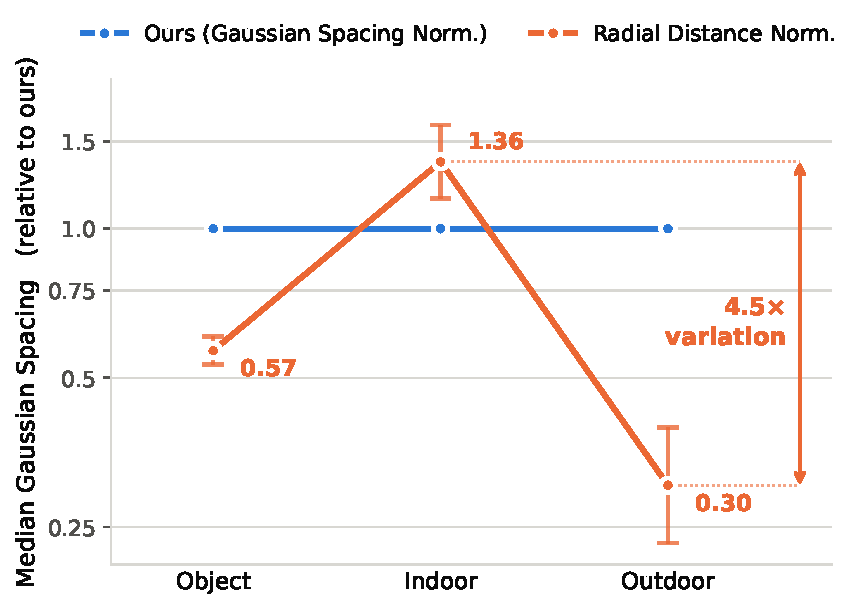
\includegraphics[width=\linewidth]{figures/method/point_spacing.pdf}
    \vspace{-0.25in}
    \caption{
        \textbf{Median Gaussian spacing across scene types.}
        RDNorm leaves up to $4.5\times$ variation in median Gaussian spacing
        across scene categories, whereas GSNorm canonicalizes it by
        construction.
    }
    \vspace{-0.1in}
    \label{fig:point_spacing_comparison}
\end{wrapfigure}

Consequently, the spacing between neighboring Gaussian centers can still
vary substantially across different scene scales and camera
configurations, as shown in
Fig.~\ref{fig:point_spacing_comparison}.
This variation is particularly
important for Gaussian prediction because the Gaussian scale required
for adequate surface coverage should be commensurate with the local
Gaussian spacing. Therefore, similar local observations can correspond
to different Gaussian-scale targets after RDNorm,
introducing ambiguity in scale supervision across scenes. This motivates us to
define the normalization space directly from a representative statistic
of Gaussian spacing.


% \vspace{-0.05in}
\paragraph{Gaussian spacing normalization.}
% \vspace{-0.05in}
We propose \emph{Gaussian Spacing Normalization (GSNorm)}, which
defines the coordinate scale for Gaussian prediction using Gaussian spacing
rather than a global radial statistic.
Because the reconstruction is rescaled by a single scene-level factor,
we use the median characteristic Gaussian spacing as a robust representative
scale.
Specifically, for a generic scene-level scale $s>0$, the characteristic
Gaussian spacing becomes
\begin{equation}
    d_i^{s}(\mathbf{u})
    \approx
    \frac{D_i(\mathbf{u})}
    {\sqrt{f_{x,i}f_{y,i}}\,s}.
\end{equation}
GSNorm chooses $s$ such that the scene-level median Gaussian spacing is
canonicalized:
\begin{equation}
    \operatorname*{median}_{i,\mathbf{u}\in\Omega_i}
    \left(
        d_i^{s}(\mathbf{u})
    \right)
    \approx
    \operatorname*{median}_{i,\mathbf{u}\in\Omega_i}
    \left(
        \frac{D_i(\mathbf{u})}
        {\sqrt{f_{x,i}f_{y,i}}\,s}
    \right)
    =
    1.
    \label{eq:gsnorm_objective}
\end{equation}

Since the median is equivariant to positive scaling,
Eq.~\ref{eq:gsnorm_objective} directly yields the normalization factor $s_g$:
\begin{equation}
    s_g
    =
    \operatorname*{median}_{i,\mathbf{u}\in\Omega_i}
    \left(
        \frac{D_i(\mathbf{u})}
        {\sqrt{f_{x,i}f_{y,i}}}
    \right).
    \label{eq:gs_scale}
\end{equation}

Using $s_g$, we rescale the geometry, depth, and camera translations as
\begin{equation}
    \mathbf{P}_i^{g}
    =
    \frac{\mathbf{P}_i}{s_g},
    \qquad
    D_i^{g}
    =
    \frac{D_i}{s_g},
    \qquad
    \mathbf{t}_i^{g}
    =
    \frac{\mathbf{t}_i}{s_g}.
    \label{eq:gsnorm}
\end{equation}

GSNorm canonicalizes the scene-level median Gaussian spacing while preserving
the relative variation of local Gaussian spacing.
This aligns the representative Gaussian spacing scale across scenes and camera
configurations without suppressing meaningful local geometric variation.
Compared with RDNorm, GSNorm therefore provides a more consistent scale
reference for Gaussian prediction that is directly related to Gaussian
surface coverage.
This alleviates ambiguity in Gaussian-scale supervision across different
input settings, facilitating the learning of a feed-forward Gaussian
model with robust cross-scene and cross-view generalization.

% \vspace{-0.1in}
\subsection{SplatAnything Architecture}
\label{sec:architecture}
% \vspace{-0.08in}
The overall architecture is illustrated in
Fig.~\ref{fig:architecture}. More details are provided in the appendix.

% \vspace{-0.1in}

\paragraph{Geometry prediction and rescaling.}

Given $N$ input images and optional camera parameters, we employ the
frozen WorldMirror~2.0~\citep{team2026hy} geometry model to estimate
multi-view depths, intrinsics, and camera poses. The predicted depths
and camera translations are initially represented in the
radial-distance-normalized coordinate space of the geometry model.
We then use GSNorm (Eq.~\ref{eq:gsnorm}) to rescale these
scale-dependent quantities into the proposed Gaussian-spacing-normalized
space, obtaining
$D^{g}=\{D_i^{g}\}_{i=1}^{N}$ and
$T^{g}=\{(R_i,t_i^{g})\}_{i=1}^{N}$.
We unproject the rescaled depth maps using the corresponding camera
parameters to obtain
$\mathbf{P}^{g}=\{\mathbf{P}_i^{g}\}_{i=1}^{N}$,
where each valid per-pixel 3D point serves as the center of a Gaussian
primitive.
% \vspace{-0.1in}

\paragraph{Gaussian attribute prediction.}

We initialize a \emph{Gaussian Backbone} from the geometry backbone
of WorldMirror~2.0 and fine-tune it for Gaussian prediction.
A lightweight \emph{GSHead}, trained from scratch, predicts
per-pixel Gaussian attributes for all input views:
\begin{equation}
    \{\mathcal{G}_i^{g}\}_{i=1}^{N}
    =
    \mathrm{GSHead}
    \left(
        \mathrm{GaussianBackbone}(\mathcal{I}, Optional\mathcal{(K, T)})
    \right).
\end{equation}

For each pixel, the network predicts opacity, rotation, scale,
and spherical-harmonic appearance coefficients.
Together with the corresponding center from $\mathbf{P}^{p}$,
these quantities define the per-pixel Gaussian primitives in the
Gaussian-spacing-normalized coordinate space.


% \paragraph{Gaussian Merging.}

% Following AnySplat~\citep{jiang2025anysplat}, we predict a per-pixel
% weight map
% $w^{p}=\{w_i^{p}\}_{i=1}^{N}$
% and merge redundant per-view Gaussians within local voxels.
% This produces the final unified 3D Gaussian scene representation
% $\mathcal{G}$.

% \vspace{-0.1in}


\subsection{Training SplatAnything}
\label{sec:training}
The training datasets and view-sampling strategies are detailed in the
appendix.

Given a rendered target-view image $\hat{I}_t$ and its ground-truth
image $I_t$, we supervise the model using a pixel-wise MSE loss and an
LPIPS perceptual loss:
\begin{equation}
    \mathcal{L}_{\mathrm{MSE}}
    =
    \frac{1}{3HW}
    \left\|
        \hat{I}_t-I_t
    \right\|_2^2,
    \qquad
    \mathcal{L}_{\mathrm{LPIPS}}
    =
    \operatorname{LPIPS}
    \left(
        \hat{I}_t,I_t
    \right).
\end{equation}

The overall objective is
\begin{equation}
    \mathcal{L}
    =
    \lambda_{\mathrm{MSE}}
    \mathcal{L}_{\mathrm{MSE}}
    +
    \lambda_{\mathrm{LPIPS}}
    \mathcal{L}_{\mathrm{LPIPS}},
\end{equation}
where
$\lambda_{\mathrm{MSE}}=\lambda_{\mathrm{LPIPS}}=1$
in our implementation.

SplatAnything is trained for 20,000 iterations on 64 NVIDIA H20 GPUs,
using 4 to 32 input views and dynamically varying the input resolution
from 504 to 1024. We use a 500-step warm-up and learning rates of
$5\times10^{-6}/2\times10^{-5}$ for the
Gaussian Backbone and GSHead.
% \vspace{-0.15in}
\section{Experiments}
\label{sec:experiments}
\begin{table*}[t]
    % Comparison averaged across 4, 8, 16, 32, and 64 input views.
% ETH3D and DTU are averaged across 4, 8, 16, and 32 input views.
\vspace{-0.15in}
\centering
\caption{Quantitative comparison across seven benchmark datasets, averaged over \textbf{4--64 input views}. The top-3 results are highlighted as \colorbox{rankfirst}{first}, \colorbox{ranksecond}{second}, and \colorbox{rankthird}{third}.}
\vspace{0.03in}
\label{tab:main_comparison_4_64view}
\setlength{\tabcolsep}{1pt}
\renewcommand{\arraystretch}{1.28}
\small
\makebox[\textwidth][c]{%
\resizebox{\textwidth}{!}{%
\begin{tabular}{clcccccccccccccc}
    \toprule
    \multirow{2}{*}{\textbf{Input}}
    & \multirow{2}{*}{\textbf{Method}}
    & \multicolumn{2}{c}{\textbf{ScanNet}}
    & \multicolumn{2}{c}{\textbf{NRGBD}}
    & \multicolumn{2}{c}{\textbf{DL3DV}}
    & \multicolumn{2}{c}{\textbf{Tanks \& Temples}}
    & \multicolumn{2}{c}{\textbf{Mip-NeRF 360}}
    & \multicolumn{2}{c}{\textbf{ETH3D}}
    & \multicolumn{2}{c}{\textbf{DTU}} \\
    \cmidrule(lr){3-4}
    \cmidrule(lr){5-6}
    \cmidrule(lr){7-8}
    \cmidrule(lr){9-10}
    \cmidrule(lr){11-12}
    \cmidrule(lr){13-14}
    \cmidrule(lr){15-16}
    & & DISTS$\downarrow$ & LPIPS$\downarrow$
    & DISTS$\downarrow$ & LPIPS$\downarrow$
    & DISTS$\downarrow$ & LPIPS$\downarrow$
    & DISTS$\downarrow$ & LPIPS$\downarrow$
    & DISTS$\downarrow$ & LPIPS$\downarrow$
    & DISTS$\downarrow$ & LPIPS$\downarrow$
    & DISTS$\downarrow$ & LPIPS$\downarrow$ \\
    \midrule
    \multirow{6}{*}{\rotatebox[origin=c]{90}{w/o Pose}}
    & AnySplat
    & 0.278 & 0.414
    & 0.236 & 0.352
    & 0.371 & 0.327
    & 0.593 & 0.737
    & 0.538 & 0.787
    & 0.278 & 0.154
    & 0.520 & 0.810 \\
    & YoNoSplat
    & 0.265 & \third{0.236}
    & 0.285 & 0.240
    & 0.375 & \third{0.219}
    & 0.424 & \second{0.338}
    & 0.405 & 0.586
    & 0.321 & \second{0.033}
    & 0.484 & 0.729 \\
    & DA3-GS
    & 0.286 & 0.305
    & \second{0.233} & \third{0.217}
    & \third{0.337} & 0.228
    & \third{0.414} & 0.380
    & \third{0.371} & \third{0.565}
    & \third{0.228} & 0.087
    & \third{0.365} & \second{0.582} \\
    & Mirror2-GS
    & \second{0.193} & \second{0.222}
    & \third{0.235} & 0.237
    & \second{0.246} & \second{0.188}
    & \second{0.306} & \third{0.351}
    & \second{0.283} & \second{0.528}
    & \second{0.205} & 0.070
    & \second{0.347} & \third{0.617} \\
    & QuerySplat
    & \third{0.236} & 0.242
    & 0.261 & \second{0.216}
    & 0.343 & 0.291
    & 0.425 & 0.393
    & 0.412 & 0.652
    & 0.290 & \first{0.031}
    & 0.424 & 0.676 \\
    & \textbf{Ours}
    & \first{0.184} & \first{0.207}
    & \first{0.195} & \first{0.183}
    & \first{0.221} & \first{0.156}
    & \first{0.252} & \first{0.299}
    & \first{0.233} & \first{0.463}
    & \first{0.147} & \third{0.049}
    & \first{0.229} & \first{0.483} \\
    \midrule
    \multirow{7}{*}{\rotatebox[origin=c]{90}{w/ Pose}}
    & DepthSplat
    & 0.288 & 0.278
    & 0.323 & 0.272
    & 0.329 & 0.191
    & 0.397 & 0.353
    & 0.561 & 0.656
    & 0.445 & 0.068
    & 0.370 & 0.598 \\
    & TokenGS
    & 0.369 & 0.272
    & 0.333 & 0.277
    & 0.375 & 0.211
    & 0.515 & 0.346
    & 0.502 & 0.716
    & 0.400 & \third{0.042}
    & 0.593 & 0.828 \\
    & tttLRM
    & 0.292 & 0.300
    & 0.320 & 0.292
    & 0.323 & 0.196
    & \third{0.390} & \third{0.342}
    & 0.350 & 0.531
    & 0.225 & 0.063
    & 0.382 & 0.599 \\
    & ReSplat
    & \third{0.272} & \third{0.240}
    & 0.284 & 0.232
    & \third{0.304} & \second{0.159}
    & 0.396 & \first{0.275}
    & \third{0.349} & \third{0.525}
    & \third{0.219} & \first{0.027}
    & 0.441 & 0.664 \\
    & DA3-GS (Pose Cond.)
    & 0.274 & 0.291
    & \third{0.238} & \third{0.227}
    & 0.311 & 0.219
    & 0.425 & 0.368
    & 0.362 & 0.556
    & 0.223 & 0.089
    & \third{0.368} & \third{0.596} \\
    & Mirror2-GS (Pose Cond.)
    & \second{0.195} & \second{0.223}
    & \second{0.231} & \second{0.226}
    & \second{0.239} & \third{0.180}
    & \second{0.304} & 0.346
    & \second{0.272} & \second{0.506}
    & \second{0.201} & 0.062
    & \second{0.315} & \second{0.532} \\
    & \textbf{Ours (Pose Cond.)}
    & \first{0.185} & \first{0.206}
    & \first{0.186} & \first{0.162}
    & \first{0.215} & \first{0.148}
    & \first{0.251} & \second{0.290}
    & \first{0.219} & \first{0.440}
    & \first{0.133} & \second{0.037}
    & \first{0.184} & \first{0.364} \\
    \bottomrule
\end{tabular}%
}%
}
\vspace{-0.05in}

    % % Comparison across seven benchmark datasets.
% Requires \usepackage{graphicx}, which is already loaded in the main file.
    \centering
    \caption{Quantitative comparison across seven benchmark datasets using \textbf{32 input views}. The top-3 results are highlighted as \colorbox{rankfirst}{first}, \colorbox{ranksecond}{second}, and \colorbox{rankthird}{third}.}
    % \vspace{0.05in}
    \label{tab:main_comparison_32view}
    \setlength{\tabcolsep}{1pt}
    \renewcommand{\arraystretch}{1.2}
    \small
    \makebox[\textwidth][c]{%
    \resizebox{\textwidth}{!}{%
    \begin{tabular}{clcccccccccccccc}
        \toprule
        \multirow{2}{*}{\textbf{Input}}
        & \multirow{2}{*}{\textbf{Method}}
        & \multicolumn{2}{c}{\textbf{ScanNet}}
        & \multicolumn{2}{c}{\textbf{NRGBD}}
        & \multicolumn{2}{c}{\textbf{DL3DV}}
        & \multicolumn{2}{c}{\textbf{Tanks \& Temples}}
        & \multicolumn{2}{c}{\textbf{Mip-NeRF 360}}
        & \multicolumn{2}{c}{\textbf{ETH3D}}
        & \multicolumn{2}{c}{\textbf{DTU}} \\
        \cmidrule(lr){3-4}
        \cmidrule(lr){5-6}
        \cmidrule(lr){7-8}
        \cmidrule(lr){9-10}
        \cmidrule(lr){11-12}
        \cmidrule(lr){13-14}
        \cmidrule(lr){15-16}
        & & DISTS$\downarrow$ & LPIPS$\downarrow$
        & DISTS$\downarrow$ & LPIPS$\downarrow$
        & DISTS$\downarrow$ & LPIPS$\downarrow$
        & DISTS$\downarrow$ & LPIPS$\downarrow$
        & DISTS$\downarrow$ & LPIPS$\downarrow$
        & DISTS$\downarrow$ & LPIPS$\downarrow$
        & DISTS$\downarrow$ & LPIPS$\downarrow$ \\
        \midrule
        \multirow{6}{*}{\rotatebox[origin=c]{90}{w/o Pose}}
        & AnySplat
        & 0.300 & 0.430
        & \second{0.232} & 0.342
        & 0.380 & 0.338
        & 0.655 & 0.811
        & 0.618 & 0.833
        & 0.241 & 0.106
        & 0.577 & 0.805 \\
        & YoNoSplat
        & 0.268 & \third{0.238}
        & 0.296 & 0.253
        & 0.382 & \third{0.225}
        & 0.430 & \second{0.342}
        & 0.400 & 0.581
        & 0.316 & \first{0.039}
        & 0.497 & 0.706 \\
        & DA3-GS
        & 0.270 & 0.282
        & 0.249 & \third{0.233}
        & 0.355 & 0.234
        & \third{0.379} & 0.358
        & \third{0.352} & \third{0.557}
        & \third{0.211} & 0.091
        & \second{0.314} & \second{0.462} \\
        & Mirror2-GS
        & \second{0.192} & \second{0.229}
        & \third{0.238} & 0.247
        & \second{0.249} & \second{0.195}
        & \second{0.312} & \third{0.352}
        & \second{0.288} & \second{0.544}
        & \second{0.204} & 0.082
        & \third{0.371} & \third{0.623} \\
        & QuerySplat
        & \third{0.231} & 0.253
        & 0.263 & \second{0.223}
        & \third{0.343} & 0.301
        & 0.428 & 0.400
        & 0.408 & 0.658
        & 0.286 & \second{0.043}
        & 0.403 & 0.627 \\
        & \textbf{Ours}
        & \first{0.181} & \first{0.205}
        & \first{0.199} & \first{0.182}
        & \first{0.223} & \first{0.154}
        & \first{0.253} & \first{0.300}
        & \first{0.231} & \first{0.460}
        & \first{0.161} & \third{0.071}
        & \first{0.234} & \first{0.455} \\
        \midrule
        \multirow{7}{*}{\rotatebox[origin=c]{90}{w/ Pose}}
        & DepthSplat
        & \third{0.238} & 0.265
        & 0.313 & 0.277
        & \third{0.316} & 0.189
        & \third{0.340} & \third{0.341}
        & 0.530 & 0.646
        & 0.232 & \first{0.035}
        & 0.373 & 0.560 \\
        & TokenGS
        & 0.374 & 0.277
        & 0.332 & 0.282
        & 0.378 & 0.213
        & 0.534 & 0.354
        & 0.519 & 0.740
        & 0.347 & \second{0.043}
        & 0.554 & 0.772 \\
        & tttLRM
        & 0.281 & 0.286
        & 0.292 & 0.250
        & \third{0.316} & 0.190
        & 0.386 & 0.346
        & 0.334 & 0.525
        & \third{0.199} & 0.066
        & 0.349 & 0.528 \\
        & ReSplat
        & 0.271 & \third{0.245}
        & 0.302 & 0.249
        & 0.328 & \second{0.170}
        & 0.368 & \first{0.263}
        & \third{0.323} & \second{0.517}
        & 0.242 & \first{0.035}
        & 0.343 & \third{0.512} \\
        & DA3-GS (Pose Cond.)
        & 0.254 & 0.259
        & \third{0.255} & \third{0.244}
        & 0.336 & 0.235
        & 0.397 & 0.354
        & 0.340 & 0.537
        & 0.202 & 0.088
        & \third{0.324} & \second{0.473} \\
        & Mirror2-GS (Pose Cond.)
        & \second{0.194} & \second{0.230}
        & \second{0.237} & \second{0.241}
        & \second{0.241} & \third{0.185}
        & \second{0.309} & 0.346
        & \second{0.277} & \third{0.523}
        & \second{0.193} & 0.070
        & \second{0.322} & 0.521 \\
        & \textbf{Ours (Pose Cond.)}
        & \first{0.184} & \first{0.212}
        & \first{0.186} & \first{0.161}
        & \first{0.213} & \first{0.147}
        & \first{0.254} & \second{0.303}
        & \first{0.219} & \first{0.452}
        & \first{0.139} & \third{0.057}
        & \first{0.185} & \first{0.357} \\
        \bottomrule
    \end{tabular}%
    }%
    }
    \vspace{-0.15in}
\end{table*}

% \vspace{-0.1in}
\subsection{Evaluation Benchmark}
Existing benchmarks are typically concentrated on a small set of datasets and evaluate interpolated target views, making it difficult to assess cross-domain and viewpoint generalization. To provide a more comprehensive evaluation, we design a new benchmark with the following properties:

% \vspace{-0.02in}

\textbf{Cross-domain and cross-scale coverage.}
We evaluate on \textbf{seven datasets}: ScanNet~\citep{dai2017scannet}, NRGBD~\citep{azinovic2022neural}, DL3DV~\citep{ling2024dl3dv}, Tanks and Temples~\citep{knapitsch2017tanks}, Mip-NeRF 360~\citep{barron2022mip}, ETH3D~\citep{schops2017multi}, and DTU~\citep{jensen2014large}. These datasets span a wide range of physical scene scales, providing a substantially broader test of cross-domain and cross-scale generalization.

% \vspace{-0.02in}

\textbf{Controlled extrapolation and observation sparsity.}
We sample context views from a compact trajectory span and select target
views using an occlusion-aware symmetric co-visibility criterion.
The input--target overlap is controlled within \textbf{0.2--0.6}, with
lower overlap corresponding to more challenging extrapolation.
We further evaluate \textbf{1/4/8/16/32/64 input views} under a fixed
context span to isolate the effect of observation density.
More details are provided in the appendix.

\begin{figure*}[t] 
    \centering
    \includegraphics[width=\textwidth]{figures/exp/main_compare.jpg}
    \vspace{-0.2in}
    \caption{Qualitative comparisons across diverse scenes and viewpoints with multi-view input.}
    \label{fig:qualitative}
    \vspace{-0.2in}
\end{figure*}


\textbf{Multi-resolution.}
Our benchmark covers a broad resolution range, from approximately \textbf{480p to 1K}, enabling evaluation under both low- and high-resolution settings.

\textbf{Compared methods.}
We evaluate two categories methods according to whether camera poses are provided. In the \emph{w/o Pose} setting, methods reconstruct the scene directly from RGB observations, including AnySplat~\citep{jiang2025anysplat}, YoNoSplat~\citep{ye2026yonosplat}, DA3-GS~\citep{lin2025depth}, Mirror2-GS~\citep{team2026hy}, and QuerySplat~\citep{li2026querysplat}.

\begin{wraptable}{r}{0.50\textwidth}
    \vspace{-0.15in}
    % Monocular comparison across seven benchmark datasets.
    \centering
    \caption{Quantitative comparison of feed-forward 3DGS methods using a \textbf{single input view}. The top-3 results are highlighted as \colorbox{rankfirst}{first}, \colorbox{ranksecond}{second}, and \colorbox{rankthird}{third}.}
    \vspace{0.01in}
    \label{tab:main_comparison_monocular}
    \setlength{\tabcolsep}{4pt}
    \renewcommand{\arraystretch}{1.15}
    \small
    \makebox[\linewidth][c]{%
    \resizebox{\linewidth}{!}{%
    \begin{tabular}{lcccccccccccccc}
        \toprule
        \multirow{2}{*}{\textbf{Method}}
        & \multicolumn{2}{c}{\textbf{ScanNet}}
        & \multicolumn{2}{c}{\textbf{NRGBD}}
        & \multicolumn{2}{c}{\textbf{DL3DV}}
        & \multicolumn{2}{c}{\textbf{Tanks \& Temples}}
        & \multicolumn{2}{c}{\textbf{Mip-NeRF 360}}
        & \multicolumn{2}{c}{\textbf{ETH3D}}
        & \multicolumn{2}{c}{\textbf{DTU}} \\
        \cmidrule(lr){2-3}
        \cmidrule(lr){4-5}
        \cmidrule(lr){6-7}
        \cmidrule(lr){8-9}
        \cmidrule(lr){10-11}
        \cmidrule(lr){12-13}
        \cmidrule(lr){14-15}
        & DISTS$\downarrow$ & LPIPS$\downarrow$
        & DISTS$\downarrow$ & LPIPS$\downarrow$
        & DISTS$\downarrow$ & LPIPS$\downarrow$
        & DISTS$\downarrow$ & LPIPS$\downarrow$
        & DISTS$\downarrow$ & LPIPS$\downarrow$
        & DISTS$\downarrow$ & LPIPS$\downarrow$
        & DISTS$\downarrow$ & LPIPS$\downarrow$ \\
        \midrule
        SHARP
        & \first{0.223} & \first{0.244}
        & \first{0.238} & \first{0.174}
        & \second{0.335} & \second{0.280}
        & \second{0.374} & \second{0.470}
        & \first{0.328} & \first{0.505}
        & \second{0.200} & \second{0.133}
        & \second{0.433} & \second{0.724} \\
        InfiniSplat
        & \third{0.266} & \third{0.280}
        & \third{0.336} & \third{0.345}
        & \third{0.527} & \third{0.596}
        & \third{0.452} & \third{0.531}
        & \third{0.505} & \third{0.654}
        & \third{0.367} & \third{0.376}
        & \third{0.562} & \third{0.754} \\
        \textbf{Ours}
        & \second{0.238} & \second{0.274}
        & \second{0.265} & \second{0.284}
        & \first{0.279} & \first{0.220}
        & \first{0.342} & \first{0.430}
        & \second{0.410} & \second{0.599}
        & \first{0.195} & \first{0.104}
        & \first{0.327} & \first{0.657} \\
        \bottomrule
    \end{tabular}%
    }%
    }
    \vspace{-0.1in}
    \par\vspace{0.1in}
    \centering
    \includegraphics[width=\linewidth]{figures/exp/main_compare_mono.jpg}
    \vspace{-0.23in}
    \captionof{figure}{Qualitative comparisons across diverse scenes and viewpoints with monocular input.}
    \label{fig:qualitative_mono}
    \vspace{-0.5in}
\end{wraptable}

In the \emph{w/ Pose} setting, camera poses are additionally provided for model input. We compare against DepthSplat~\citep{xu2025depthsplat}, TokenGS~\citep{ren2026tokengs}, tttLRM~\citep{wang2026tttlrm}, ReSplat~\citep{xu2025resplat}, as well as pose-conditioned variants of DA3-GS~\citep{lin2025depth} and Mirror2-GS~\citep{team2026hy}.
Additionally, we compare against SHARP~\citep{mescheder2026sharp} and InfiniSplat~\citep{wang2026infinisplat}, which target for monocular view synthesis.

% \vspace{-0.1in}
\subsection{Quantitative Comparisons}
% \vspace{-0.07in}

We report the average metrics over \textbf{4/8/16/32/64 input views} in Table~\ref{tab:main_comparison_4_64view}, specific results under different input-view settings are provided in the appendix. Following SHARP~\citep{mescheder2026sharp}, we primarily report \textit{LPIPS} and \textit{DISTS} in the main paper, as they better reflect rendering quality and higher-frequency details. We also report the results in the monocular setting in Table~\ref{tab:main_comparison_monocular}.
Overall, SplatAnything achieves the strongest performance across most datasets and evaluation settings, demonstrating its superior generalization capabilities.

% \vspace{-0.1in}
\subsection{Qualitative Comparisons}
% \vspace{-0.1in}

Figs.~\ref{fig:qualitative} and~\ref{fig:qualitative_mono} present qualitative comparisons across diverse scenes and extrapolated viewpoints under multi-view and monocular input settings, covering object-centric captures, indoor environments, and large-scale outdoor scenes. \textbf{SplatAnything} demonstrates a significant advantage in rendering quality: it generalizes robustly across a wide range of scene types and spatial scales, maintains geometric consistency under challenging large viewpoint
extrapolation, and produces sharp, detailed renderings that faithfully recover fine local structures. More results are provided in the appendix.
% \vspace{-0.08in}
\subsection{Efficiency Analysis}
% \vspace{-0.08in}
We evaluate the inference efficiency of \textbf{SplatAnything} and other methods under different input-view settings. Detailed timing results are provided in the appendix.

% \vspace{-0.08in}
\subsection{Ablation Studies}
% \vspace{-0.06in}
\paragraph{Effect of Gaussian spacing normalization.}
We ablate the normalization space for Gaussian prediction in
Table~\ref{tab:ablation_normalization_space}, comparing RDNorm,
RDNorm with scale calibration, and GSNorm under the same architecture
and training settings.
For RDNorm with scale calibration, Gaussian prediction remains in the
RDNorm space, while the predicted Gaussian scales are uniformly rescaled
to match the scene's median Gaussian spacing. Both RDNorm variants remain consistently inferior to GSNorm.
Qualitatively, RDNorm tends to produce holes in small object-centric
scenes and over-smoothed results in large outdoor scenes
(Fig.~\ref{fig:ablation}).
Scale calibration alleviates the holes on object-centric scenes, but
often turns them into over-smoothed reconstructions, while outdoor scenes
remain blurry.
These results indicate that post-prediction scale correction cannot
resolve the ambiguity in scale supervision introduced by RDNorm.
By canonicalizing the representative Gaussian spacing scale before Gaussian
prediction, GSNorm provides a better-aligned prediction space and yields
more complete and sharper reconstructions across diverse scenes. 
Additional results are provided in the appendix.

% \vspace{-0.1in}
\paragraph{Training design choices}
We also analyze several architecture and training design choices, including
fine-tuning the pretrained geometry backbone, fixing Gaussian centers,
scaling the amount of training data, and using mixed sampling strategies
for Gaussian supervision. Please refer to the appendix for more analysis and results.

% Ablation study on the choice of normalization space.
% Replace ``--'' with the corresponding experimental results.
\vspace{-0.04in}
\begin{table*}[t]
    \centering
    \caption{Normalization-space ablation across different numbers of input views.}
    \vspace{0.02in}
    \label{tab:ablation_normalization_space}
    \setlength{\tabcolsep}{4pt}
    \renewcommand{\arraystretch}{1.05}
    \small
\makebox[\textwidth][c]{%
\resizebox{\textwidth}{!}{%
    \begin{tabular}{lcccccccccccc}
        \toprule
        \multirow{2}{*}{\textbf{Norm. Space}}
        & \multicolumn{2}{c}{\textbf{Num. Views=1}}
        & \multicolumn{2}{c}{\textbf{Num. Views=4}}
        & \multicolumn{2}{c}{\textbf{Num. Views=8}}
        & \multicolumn{2}{c}{\textbf{Num. Views=16}}
        & \multicolumn{2}{c}{\textbf{Num. Views=32}}
        & \multicolumn{2}{c}{\textbf{Num. Views=64}} \\
        \cmidrule(lr){2-3}
        \cmidrule(lr){4-5}
        \cmidrule(lr){6-7}
        \cmidrule(lr){8-9}
        \cmidrule(lr){10-11}
        \cmidrule(lr){12-13}
        & DISTS$\downarrow$ & LPIPS$\downarrow$
        & DISTS$\downarrow$ & LPIPS$\downarrow$
        & DISTS$\downarrow$ & LPIPS$\downarrow$
        & DISTS$\downarrow$ & LPIPS$\downarrow$
        & DISTS$\downarrow$ & LPIPS$\downarrow$
        & DISTS$\downarrow$ & LPIPS$\downarrow$ \\
        \midrule
        Radial Distance Norm.
        & 0.308 & 0.394
        & 0.223 & 0.278
        & 0.223 & 0.272
        & 0.218 & 0.268
        & 0.225 & 0.277
        & 0.224 & 0.250 \\
        Radial Distance Norm + Scale Calibration.
        & 0.323 & 0.400
        & 0.249 & 0.309
        & 0.252 & 0.308
        & 0.245 & 0.300
        & 0.253 & 0.305
        & 0.234 & 0.265 \\
        \textbf{Gaussian Spacing Norm. (Ours)}
        & \textbf{0.294} & \textbf{0.367}
        & \textbf{0.198} & \textbf{0.245}
        & \textbf{0.196} & \textbf{0.237}
        & \textbf{0.190} & \textbf{0.232}
        & \textbf{0.197} & \textbf{0.241}
        & \textbf{0.217} & \textbf{0.229} \\
        \bottomrule
    \end{tabular}%
}%
}
\end{table*}
% \vspace{-0.2in}
\begin{figure*}[t] 
    \centering
    \vspace{-0.1in}
    \includegraphics[width=\linewidth]{figures/exp/ablation.jpg}
    \vspace{-0.25in}
    \caption{Ablation studies on the effect of GSNorm across different scene types.}
    \label{fig:ablation}
    \vspace{-0.12in}
\end{figure*}

% Quantitative and qualitative results are shown in Tab.~\ref{tab:ablation_training_design_choices} and Fig.~\ref{fig:ablation_training_design_choices}. We find that finetuning the pretrained geometry backbone brings improvements. Fixing the gaussian centers ensures more correct geometry across viewpoint changes, as RGB-projection loss tends to overfit the geometry to the input views. Also, using mixed sampling strategies for training feed-forward Gaussian Splatting can learn more reaonable Gaussian attributes, especially under the extrapolation viewpoint shifts.




\section{Conclusion}

\label{sec:conclusion}
We identified a key limitation of existing methods: \emph{Radial Distance
Normalization (RDNorm)} does not directly normalize Gaussian spacing,
leading to ambiguity in Gaussian-scale supervision across scene scales and
camera configurations. To address this issue, we introduced
\textbf{SplatAnything} with \textit{Gaussian Spacing Normalization (GSNorm)},
which derives a scene-level normalization factor from a representative
statistic of Gaussian spacing and provides a more consistent spatial
reference for Gaussian prediction. We further established a systematic
cross-dataset benchmark covering different input sparsity levels and
challenging extrapolated viewpoints. Experiments demonstrate that
SplatAnything achieves the strongest performance across most evaluation
settings, highlighting the effectiveness of GSNorm and marking a
substantial step toward feed-forward 3DGS.

\paragraph{Limitations and Future Work.}
SplatAnything relies on geometric priors from a geometry foundation model
and may degrade when reliable geometry cannot be recovered from extremely
sparse or challenging inputs. It also primarily reconstructs regions
visible in the input views, which can leave holes in unobserved areas.
Future work will explore more robust geometry estimation and generative
priors for completing unobserved regions.

\subsection*{AI use statement}

In this work, we used generative AI tools to assist with writing, language
polishing, and code development. In particular, generative AI was used to
improve the clarity, grammar, and presentation of the manuscript, and to
assist with parts of code implementation and debugging under the authors'
direction. All AI-assisted text was carefully reviewed and revised by the
authors, and all AI-assisted code was manually inspected, tested, and
verified for correctness.
Generative AI was not used to independently originate the research ideas,
formulate the research questions, or design the core technical
contributions of this work. We also did not use generative AI tools to
generate experimental or training data, or to independently search for,
select, or determine the references used in the paper. The authors take
full responsibility for the final content of this work, including all
text, technical claims, experimental results, and code produced with the
assistance of generative AI.

% Temporary: keep BibTeX compilable while the section files contain no citations.
% Remove this line after adding the first real \cite command.
\nocite{*}

\bibliography{iclr2027_conference}
\bibliographystyle{iclr2027_conference}

\input{sec/11_appendix}

\end{document}
